
{
    In the development of any engineering system, a fundamental aspect is the measurement of its performance. 
    In this project, we have one primary system, the \ac{MOT} tracker, along with two subsystems: the object detector and the appearance model. 
    Each of these components has its own set of evaluation metrics to quantify its performance
}

\subsubsection{Object Detection Metrics}

{
    An object detector solves the object localization and classification problems at the same time. 
    This kind of problem is evaluated by the precision, recall, F1-Score and \ac{mAP} metrics.
}

{
    These metrics require the definition of true positives, false positives and false negatives:
}

\begin{itemize}
    \item The \textbf{true positives} (\acs{TP}) are defined by correctly matching a class detections with ground truth objects of the same class. Usually a \ac{IoU} threshold is used to match the detections, similar to the association step of a SORT tracker.
    \item The \textbf{false positives} (\acs{FP}) are defined by incorrectly assigning a class on the detected object, it applies to matched objects and detected background.
    \item The \textbf{false negatives} (\acs{FN}) are defined by the absence of matching detections for ground truth objects.
\end{itemize}

\paragraph{Precision}

{
    Precision is a metric that measures the correctness of the detected set, a high precision means a high certainty on the detected objects, however it does not contemplate undetected objects.
}

\paragraph{Recall}

{
    Recall is a metric that measures the ability to detect targets, a high recall means a high certainty on detecting the relevant objects, however it does not contemplate undesired detections.
}

%\begin{figure}[!ht]
%    \centering
%    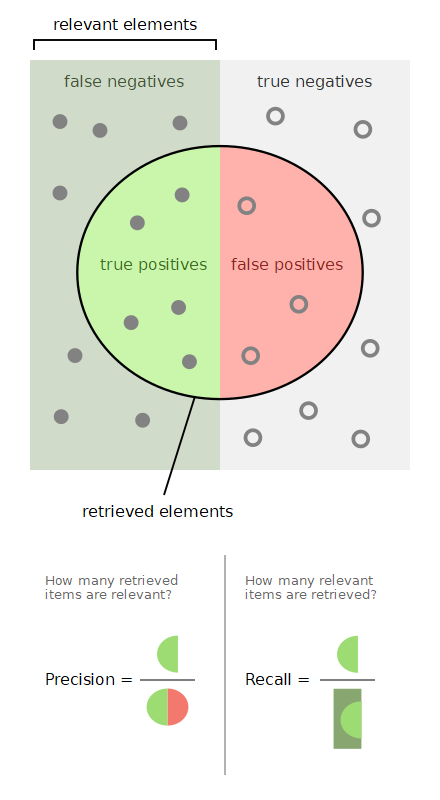
\includegraphics[width=0.3\linewidth]{figures/05_methodology/Precisionrecall.png}
%    \caption[Precision and recall]{\footnotesize{Visual representation of precision and recall extracted from WikipediaCommons\cite{precision_recall}.}}
%    \label{fig:precision and recall}
%\end{figure}
%
%{
%    Figure \ref{fig:precision and recall} describes graphically and mathematically precision and recall.
%}

\paragraph{F1-Score}

{
    F1-Score is the harmonic mean of precision and recall which symmetrically represents both metrics, it allows a good global evaluation of a model. 
%    Its formula is the following:
}

%\begin{equation}
%    \label{eqn:F1Score}
%    F_{1} = 2 \cdot \frac{precision \cdot recall}{precision + recall}
%\end{equation}

%{
%    Usually, deep learning based detection models return their confidence score. 
%    F1-Score, precision and recall computed on a validation dataset can be used to determine that parameter.
%    There is a compromise between precision and recall that makes the choice of a good threshold a non-trivial task.
%}

\paragraph{Mean Average Precision}

{
    \ac{AP} and \acl{mAP} (\ac{mAP}) are other global performance metrics like F1-Score. 
    \ac{AP} join precision and recall regardless of the confidence threshold for a given class. 
    \Ac{mAP} averages the \ac{AP} metric across multiple outputs generated by various user-defined settings. 
    These sets of outputs are referred to as queries.
}

{
    The most popular conventions for the \ac{mAP} set of settings are the isolation of each class and the definition of multiple \ac{IoU} threshold used to match the detections with the ground truth. 
    This project only detects one class, which means that only the \ac{IoU} threshold is modified.
}

%{
%    The \ac{AP} metric is obtained by averaging the precision curve ($P(R)$) in function of the recall ($R$) from 0 to 1:
%}

%\begin{equation}
%    \label{eqn:AP theory}
%    AP = \int_{0}^{1} P(R) \, dR
%\end{equation}

%{
%    In practice, the precision and recall curve is estimated by a given dataset becoming a set of not equidistributed points. 
%    In order to average the precision and recall curve, the data output is sorted by decreasing confidence (the $i-th$ detection is ranked $k_{i}$), the precision is computed within a subset of the $k$ more confident detections ($P(k)$) and, at the end, each ranked precision is weighted averaged by the width of the recall interval from the previous rank to the current rank.
%}

%\needspace{0.1\textheight}

{
%    The mathematical expression of the defined weighted average can be simplified into the simple mean of the ranked precision of the ground truth elements, with the false negatives redefined to have a ranked precision of 0:
    The \ac{AP} metric is obtained by averaging the precision in function of the recall curve. In practice, an estimation is obtained by a weighted average that can be simplified into the simple mean of the ranked precision of the ground truth elements, with the false negatives redefined to have a ranked precision of 0:
}

\begin{equation}
    \label{eqn:AP real}
    AP = \frac{\mathlarger{\sum\limits_{i \in TP}} P(k_{i})}{|TP| + |FN|}
\end{equation}

{
    This project uses the \textbf{\ac{mAP}@50} (or \ac{AP}@50 because there is only one class) and the \textbf{\ac{mAP}@50-95}. 
    The @ notation refers to the \ac{IoU} threshold queries, being \textbf{\ac{mAP}@50} the \ac{AP} when the \ac{IoU} is set to 0.5 and \textbf{\ac{mAP}@50-95} the mean of the \ac{AP} computed with \ac{IoU} thresholds of 0.5, 0.55, 0.6, 0.65, 0.7, 0.75, 0.8, 0.85, 0.9 and 0.95.
}

\subsubsection{Identity Re-identification Metrics}

{
    An appearance model solves the identity re-identification problem. 
    This kind of problem is evaluated by the rank metrics and the already seen \textbf{\ac{mAP}} using the identities on the desired validation dataset classes as queries.
}

{
    In re-identification problems true negatives can also be defined, in addition to true positives, false positives and false negatives:
}

\begin{itemize}
    \item The \textbf{true positives} are defined by correctly matching pairs of ants images with the same identity.
    \item The \textbf{true negatives} (\acs{TN}) are defined by correctly not matching pairs of ants images with different identities.
    \item The \textbf{false positives} are defined by incorrectly matching pairs of ants images with different identities.
    \item The \textbf{false negatives} are defined by incorrectly not matching pairs of ants images with the same identities.
\end{itemize}

\paragraph{Rank metrics}

{
    The $k$-rank metrics redefine true positives (${TP}_{k}$) by the existence on any correct match for a query ant within the $k$ nearest appearances.
    The final metric is the accuracy of the given set of queries:
}

\begin{equation}
    \label{eqn:rank accuracy}
    Rank_{k} = \frac{|{TP}_{k}|}{|queries|}
\end{equation}

{
    This project contemplates the rank-1 metric or accuracy.
}

\needspace{0.15\textheight}

\subsubsection{Multiple Object Tracking Metrics}

{
    Evaluating multiple object tracking is a complex problem comparable to the tracking task itself. 
    The reason of this complexity is the fact that a tracking system solves 3 problems:
}

\begin{itemize}
    \item \textbf{Detection}: the target objects are found. % independently of the identity. but the matching score priorize identity to get TP anyway
    \item \textbf{Localization}: the found objects are spatially aligned with their target. % independently of the identity. but the matching score priorize identity to get TP anyway
    \item \textbf{Association}: the found objects are temporally aligned with their target identity.
\end{itemize}

{
    For this reason, there exist a lot of metrics that prioritize one problem over the others or evaluate each problem with different criteria.
    In this project, it was decided to use the \ac{HOTA}\cite{luiten2020IJCV} group of metrics because the authors of these metrics states that the \ac{HOTA} metric, that jointly evaluates the three problems, is balanced with respect the three problems (see Figure \ref{fig:hota_vs_others}).
}

\begin{figure}[!h]
    \centering
    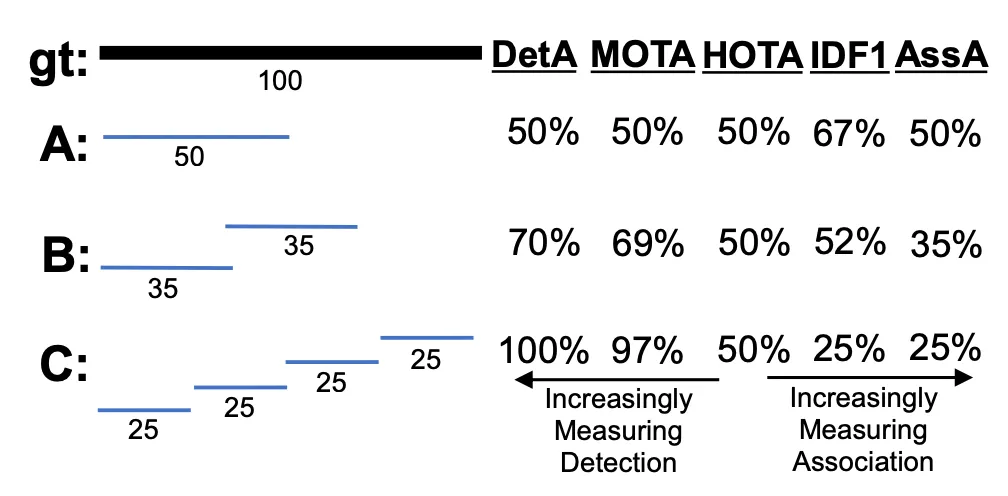
\includegraphics[width=0.75\linewidth]{figures/05_methodology/HOTA_vs_other.png}
    \caption[HOTA compared with other metrics]{\footnotesize{
        Image extracted from the HOTA paper\cite{luiten2020IJCV}. \\
        HOTA, DetA and AssA compared with other popular metrics (MOTA\cite{MOTA} and IDF1\cite{ristani2016performance}).
        }}
    \label{fig:hota_vs_others}
\end{figure}

{
    Similar to the other metrics, the first step is the definition of true positives, false negatives and false positives. 
    However, to obtain these values, a matching between ground truth and tracks is required.
    This matching should aim to maximize the final metric while maintaining plausibility. 
    The rationale behind this criterion is that all consistent interpretations of the system's output that align with the ground truth are valid, 
    and the maximized interpretation is likely the most accurate.
}

{
    The authors of \ac{HOTA} solve this optimization problem with the Hungarian algorithm using a composed score. The score uses a \textbf{current frame} spatial similarity component and a \textbf{global} estimated ``optimal association" score.
    The estimated association score is a prematching proxy for an association score that approaches the estimated one for the optimal assignment.
}

{
    The spatial similarity can be the previously explained \ac{IoU}, the previous ``plausibility'' refers to a threshold value applied on this score after the ground truth matching. 
}

{
    The estimated association score is a multiple frames Jaccard index\footnote{The Jaccard index is the intersection of two sets over their union (\ac{IoU}).}, it is computed as the available spatial associations (with a higher spatial similarity than the threshold) of a pair ``ground truth identity''-``tracked object identity'' for all the frames over the number of frames where at least one of the identities was present (see Figure \ref{fig:hota_preassociation}).
}

\begin{figure}[!h]
    \centering
    
\includegraphics[width=\linewidth]{figures/05_methodology/HOTA_association_example.png}
    \caption[HOTA: Track overlap with ground truth]{\footnotesize{
        This image illustrates a case where a track of 3 frames overlaps during 2 frames with a ground truth identity of 4 frames. 
        The denominator of the estimated optimal association will be 3-2+4=5. 
        The numerator can be 2 for a threshold smaller than 0.5, 1 for a threshold smaller than 0.8 and 0 for a threshold higher than 0.8. 
        With a threshold of 1 the association score cannot be different than the estimated association score.
        }}
    \label{fig:hota_preassociation}
\end{figure}

{
    Once the spatial similarity ($\mathcal{S}$), the estimated association score ($\mathcal{A}_{max}$) and the similarity threshold ($\alpha$) are defined, the potential matching score used for the linear assignment joins them as in the equation \ref{eqn:potential matching score}:
}

\begin{equation}
    \label{eqn:potential matching score}
    MS(i, j) = \begin{cases}
        \frac{1}{\varepsilon} + \mathcal{A}_{max}(i, j) + \varepsilon \cdot \mathcal{S}(i, j) & \text{if } \mathcal{S}(i, j) \geq \alpha\\
        0 & \text{otherwise}
    \end{cases}
\end{equation}
    
{
    The matching algorithm was implemented in order to use the ground truth to analyses our results and test the viability of a model.
}

{
    With a mapping between ground truth and output tracks, \ac{HOTA} defines true positives, false negatives, false positives:
}

\begin{itemize}
    \item The \textbf{true positives} are detections that are matched with a ground truth object, independently of the identity, it measures the performance of the detection and localization problems.
    \item The \textbf{false negatives} are ground truth objects that are not matched.
    \item The \textbf{false positives} are detections that are not matched.
\end{itemize}

{
    Additionally, \ac{HOTA} defines new values called true positives associations (\acs{TPA}), false negatives associations (\acs{FNA}) and false positives associations (\acs{FPA}).
    The \ac{TPA}, \ac{FNA} and \ac{FPA} are defined independently over all the pairs of ``ground truth identity''-``tracked object identity'' within the true positives set; a single evaluation has got one set of true positives, false negatives and false positives and $C=|TP|$ sets of true positives associations, false negatives associations and false positives associations. 
    These values measure the performance of the association problem:
}
\begin{samepage}
    \begin{itemize}
        \item The \textbf{true positives associations}, given a true positive of interest ``c", are all the true positives which have the same ``ground truth identity''-``tracked object identity'' pairs than the interest true positive ``c"; all \ac{TPA}s have the same \ac{TPA}, \ac{FNA} and \ac{FPA} which reduce the number of computation although the concept is defined for all the \ac{TP}s.
        \item The \textbf{false negatives associations}, given a true positive of interest ``c", are the ground truth objects with the same identity as the ground truth from ``c'' that were not assigned the tracked object identity from ``c'' (different or unassigned identities).
        \item The \textbf{false positives associations}, given a true positive of interest ``c", are the detections with the same identity as the detection from ``c'' that were not assigned the ground truth identity from ``c'' (different or unassigned identities).
    \end{itemize}
\end{samepage}

{
    With the new association measures, the previously mentioned association score can be properly defined:
}

\begin{equation}
    \label{eqn:association score}
    \mathcal{A}(C) = \frac{|TPA(c)|}{|TPA(c)| + |FNA(c)| + |FPA(c)|}
\end{equation}

\paragraph{\ac{HOTA}\textsubscript{$\alpha$}}

{
    \ac{HOTA}\textsubscript{$\alpha$} is a metric defined by a double Jaccard formulation, where the association score ($\mathcal{A}$) is a Jaccard metric over the associations that weights the true positives of a Jaccard metric over the detection concept. 
    And $\alpha$ is the threshold on location similarity.
}

\begin{equation}
    \label{eqn:hota alpha}
    HOTA_{\alpha} = \sqrt{\frac{\sum_{c \in \{TP\}} \mathcal{A}(c)}{|TP| + |FN| + |FP|}}
\end{equation}

{
    The square root is needed because the dimensionality of the summation of association scores (multiplied by true positive of value 1) is squared (jointly detection domain and association domain) over unsquared (association domain), and the detection Jaccard makes the denominator squared (jointly detection domain and association domain).
}

\paragraph{\ac{HOTA}}

{
    Theoretically, \ac{HOTA} is the average of $HOTA_{\alpha}$ on all the location similarity domain (from 0 to 1). In practice, it can be approximated by a mean:
}

\begin{equation}
    \label{eqn:hota}
    \text{HOTA} = \int_{0}^{1} \text{HOTA}_{\alpha} \, d\alpha \approx \frac{1}{19} \cdot \sum_{\alpha \, \in \, \{0.05 \cdot i \,|\, 1 \leq i \leq 19\}} \text{HOTA}_{\alpha}
\end{equation}

\paragraph{LocA}

{
    Localization Accuracy (\ac{LocA}) is a measure of localization that average the different localization thresholds:
}

\begin{equation}
    \label{eqn:loca}
    \text{LocA} = \int_{0}^{1} \frac{1}{|\text{TP}_{\alpha}|} \cdot \sum_{c \, \in \, \{\text{TP}_{\alpha}\}} \mathcal{S}(c) \, d\alpha
\end{equation}

\paragraph{DetA}

{
    Detection Accuracy (\ac{DetA}) is the detection Jaccard index with a given localization threshold $\alpha$. It can be further decomposed into detection precision and detection recall but it is not used in this project.
}

\begin{equation}
    \label{eqn:deta}
    \text{DetA}_{\alpha} = \frac{|\text{TP}_{\alpha}|}{|\text{TP}_{\alpha}| + |\text{FN}_{\alpha}| + |\text{FP}_{\alpha}|}
\end{equation}

\paragraph{AssA}

{
    Association Accuracy (\ac{AssA}) is a measure of association that average the association score with a given localization threshold $\alpha$.
}

\begin{equation}
    \label{eqn:assa}
    \text{AssA}_{\alpha} = \frac{1}{|\text{TP}_{\alpha}|} \cdot \sum_{c \, \in \, \{\text{TP}_{\alpha}\}} \mathcal{A}(c) \, d\alpha
\end{equation}

{
    Another interpretation of \ac{HOTA}\textsubscript{$\alpha$} is the geometric mean of \ac{DetA}\textsubscript{$\alpha$} and \ac{AssA}\textsubscript{$\alpha$}.
}
